\chapter{Circular Motion}

\section{Angular quantities}

Movement or rotation of an object along a circular path is called \keypoint{circular motion}, to describe a circular motion, we can use \emph{angular quantities}, which turn out to be more useful than linear displacement , linear velocity , etc.


\subsection{Angular displacement}

\begin{ilight}
	\keypoint{Angular displacement}\index{angular displacement} is angle swiped out by object moving along circular
\end{ilight}

\begin{marginfigure}
	\centering
	\vspace*{-8pt}
	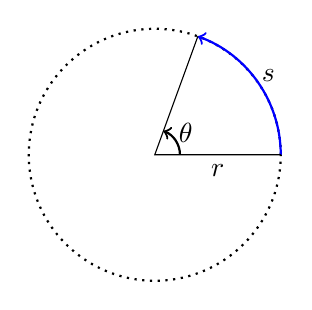
\begin{tikzpicture}[scale=0.8]
		\draw[dotted,thick] (0,0) circle(2);
		\draw[->,thick,blue] (2,0) arc (0:70:2);
		\draw (2,0) -- (0,0) node[midway,below]{$r$} -- (70:2);
		\draw[->,thick] (0.4,0) arc (0:70:0.4);
		\node at (35:0.6) {$\theta$};
		\node at (35:2.2) {$s$};
	\end{tikzpicture}
\end{marginfigure}

unit: $[\theta]=\rad \quad$ (natural unit of measurement for angles)

conversion rule: $2\pi \rad = 360^\circ$

\cmt if two radii form an angle of $\theta$, then length of arc: $s=r\theta$

two radii subtending an arc of same length as radius form an angle of one \keypoint{radian}\index{radian}


\subsection{Angular velocity}

Angular velocity describes how fast an object moves along a circular path

\begin{ilight}
	\keypoint{Angular velocity}\index{angular velocity} is defined as angular displacement swiped out per unit time: $\tcbhighmath{\omega = \frac{\Delta \theta}{\Delta t}}$
\end{ilight}

\cmt unit of: $[\omega] = \radps$, also in radian measures

\cmt angular velocity is a \emph{vector} quantity that points in a direction normal to the plane of circular motion but in A-level course, we treat angular velocity as if it is a scalar. Angular velocity and angular speed may be considered to be the same idea

Angular and linear velocity are closely related: in interval $\Delta t$, distance moved along arc $$\Delta s=v\Delta t=r \Delta\theta \RA \omega = \frac{\Delta \theta}{\Delta t} = \frac{v}{r} \RA \tcbhighmath{v=\omega r}$$

this relation between linear speed and angular speed holds at any instant


\subsection{Uniform circular motion}

Consider the simplest possible circular motion $\longrightarrow$ circular motion with constant $\omega$

\begin{marginfigure}
	\centering
	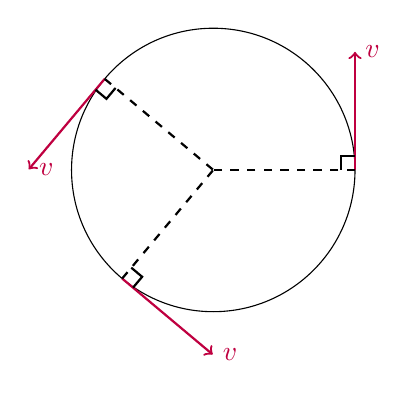
\begin{tikzpicture}[scale=0.6]
	\draw (0,0) circle [radius=3];
	\foreach \s in {0,140,230}
	{
		\draw [purple, thick, ->] (\s:3) -- ++(\s+90:2.5) node[right]{$v$};
		\draw [thick, dashed] (\s:3) -- (0,0);
		\draw [thick] (\s:2.7) -- ++(\s+90:0.3) -- ++(\s:0.3);
	}
	\end{tikzpicture}
\end{marginfigure}

analogy with linear motion with constant $v$

uniform linear motion: $s=vt$

displacement $s \leftrightarrow \theta$, velocity $v \leftrightarrow \omega$

for uniform circular motion, one has: $$\tcbhighmath{\theta=\omega t}$$

\cmt time taken for one complete revolution is called \keypoint{period} $T$

in one $T$, angle swiped is $2\pi$, so $$\tcbhighmath{\omega=\frac{2\pi}{T}}$$

\cmt uniform circular motion is still \emph{accelerated} motion

speed is unchanged, but \emph{velocity} is changing

direction of velocity always \emph{tangential} to its path, so direction of velocity keeps changing

in general, any object moving along circular path is accelerating

\example{An object undergoes a uniform motion around a circular track of radius 2.5 m in 40 s, what is its angular speed and linear speed?}

\begin{soln}
    


\begin{equation*}
	\omega = \frac{2\pi}{T} = \frac{2\pi}{40} \approx 0.157 \radps \qquad v = \omega r = 0.157 \times 2.5 \approx 0.39 \mps 
\end{equation*}
\end{soln}

\question{What is the angular velocity of the minute hand of a clock?}

\question{A spacecraft moves around the earth in a circular orbit. The spacecraft has a speed of $7200 \mps$ at a height of 1300 km above the surface of the earth. Given that the radius of the earth is 6400 km. (a) What is the angular speed of this spacecraft? (b) What is its period?}


\subsection{Centripetal acceleration}

\rcyskip

\begin{ilight}
	\keypoint{Centripetal acceleration} is the acceleration due to the change in direction of velocity vector, it points toward the centre of circular path
\end{ilight}

consider motion along a circular path from $A$ to $B$ with constant speed $v$

under small (infinitesimal) duration of time $\Delta t$\footnote{A more rigorous derivation can be given by using differentiation techniques}

\begin{figure}[ht]
	\centering
		\begin{tikzpicture}[scale=1]
		\draw [thick, dashed] (70:4) arc [radius=4, start angle=70, end angle=110];
		\draw [thick] (80:1.5) arc [radius=1.5, start angle=80, end angle=100];
		\foreach \s in {80,100}
		{
			\draw [purple, thick, ->] (\s:4) -- ++(\s-90:1.2) node[above]{$v$};
			\draw [thick, dashed] (\s:4) -- (0,0);
		}
		\draw (80:4) node[above]{$B$};
		\draw (100:4) node[above]{$A$};
		\draw (0,1.5) node[above]{$\Delta \theta$};
		\draw [thick,->] (2.5,2) --++ (2,0);
		\draw [purple, thick, ->] (5.5,2) -- ++(10:1) node[above] {$v$} -- ++(10:1);
		\draw [purple, thick, ->] (5.5,2) -- ++(-10:1) node[below] {$v$} -- ++(-10:1);
		\draw [purple, thick, ->] (7.470,2.347) -- ++ (0,-0.347) node[right]{$\Delta v$} -- ++ (0,-0.347);
		\draw (5.6,1.9) node[below]{$\Delta \theta$};
		\draw (5.5,2) ++ (-10:0.5) arc(-10:10:0.5);
		\end{tikzpicture}
\end{figure}


	change in velocity: $\Delta v = 2v\sin\frac{\Delta \theta}{2} \approx v \Delta \theta \quad$ (as $\Delta \theta \to 0$, $\sin \Delta \theta \approx \Delta \theta$)
	
	acceleration: $a = \frac{\Delta v}{\Delta t} \approx v \frac{\Delta \theta}{\Delta t} = v \omega \quad$ (as $\omega = \frac{\Delta \theta}{\Delta t}$)
	
	recall relation $v = \omega r$, we find centripetal acceleration: $$\tcbhighmath{a_c = \frac{v^2}{r} = \omega^2 r}$$\index{centripetal acceleration}

\cmt direction of centripetal acceleration: always towards centre of circular path
	
\cmt centripetal acceleration is only responsible for the change in \emph{direction} of velocity

change in \emph{magnitude} of velocity will give rise to \emph{tangential acceleration}

this is related to \emph{angular acceleration}\footnote{Angular acceleration is analogous to linear acceleration $\alpha$, defined as rate of change of angular velocity: $\alpha = \frac{\dd \omega}{\dd t} = \frac{\dd^2 \theta}{\dd t^2}$ \piste. Similar to $v=\omega r = \ddt{s}$, the relation $a=\alpha r = \ddt{v}$ also holds.}  , which is beyond the syllabus

\question{A racing car makes a $180^\circ$ turn in 2.0 s. Assume the path is a semi-circle with a radius of 30 m and the car maintains a constant speed during the turn. (a) What is the angular velocity of the car? (b) What is the centripetal acceleration?}

\subsection{Centripetal force}

Circular motion must involve change in velocity, so object is not in equilibrium 

there must be a \emph{net force} on an object performing circular motion 

\begin{ilight}
	\keypoint{Centripetal force}\index{centripetal force} ($F_c$) is the resultant force acting on an object
	moving along a circular path, and it is always directed towards centre of the circle
\end{ilight}

\cmt centripetal force causes centripetal acceleration

using Newton's 2$^\text{nd}$ law: $$\tcbhighmath{ F_c = m\frac{v^2}{r} = m\omega^2r}$$

\cmt $F_c$ is not a new force by nature, it can have a variety of origins

$F_c$ is a resultant of forces you learned before (weight, tension, contact force, friction, etc.)

\cmt $F_c$ acts at right angle to direction of velocity

or equivalently, if $\fnet \perp v$ and $\fnet$ is of constant magnitude

then this net force provides centripetal force for circular motion

\cmt effect of $F_c$: change \emph{direction} of motion, or maintain circular orbits

to change \emph{magnitude} of velocity, there requires a \emph{tangential} component for the net force

again the idea of tangential force is beyond the syllabus

\example{Planet orbiting around a star}
\begin{soln}
\begin{center}
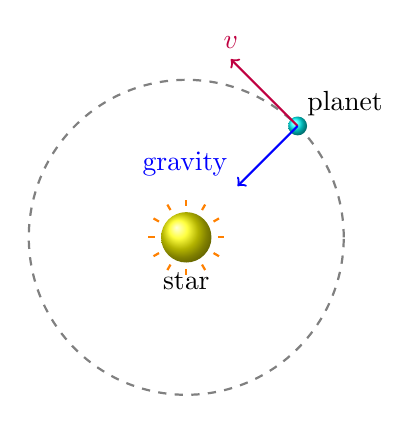
\begin{tikzpicture}[scale=0.8]
\shade [ball color = yellow] (0,0) circle (0.4);
\node at (0,-0.7){star};
\foreach \s in {0,30,60,...,330}
 \draw [orange, thick] (\s:0.5) -- ++(\s:0.1);
\draw [gray, thick, dashed] (0:2.5) arc [radius=2.5, start angle=0, end angle=360];
\shade [ball color = Cyan] (45:2.5) node[above right]{planet} circle (0.15);
\draw [purple, thick, ->] (45:2.5) -- ++(135:1.5) node[above]{$v$};
\draw [thick, ->, blue] (45:2.5) -- ++(225:1.35) node[above left]{gravity};
\end{tikzpicture}
\end{center}
gravity by the star provides centripetal force for the planet
\end{soln}


\example{A rock is able to orbit around the earth near the earth's surface. Let's ignore air resistance for this question, so the rock is acted by weight only. Given that radius of the earth $R=6400$ km. (a) What is the orbital speed of the rock? (b) What is the orbital period?}
	
\begin{soln} weight of object provides centripetal force: $mg = \frac{mv^2}{R}$
	
orbital speed: $v = \sqrt{gR} = \sqrt{9.81\times6.4\times10^6} \approx 7.9\times10^3 \mps$

period: $T = \frac{2\pi R}{v} = \frac{2\pi\times6.4\times10^6}{7.9\times10^3} \approx 5.1\times10^3 \text{ s} \approx 85 \text{ min}$ \end{soln}

\example{A turntable can rotate freely about a vertical axis through its centre. A small object is placed on the turntable at distance $d=40$ cm from the centre. The turntable is then set to rotate, and the angular speed of rotation is slowly increased. The coefficient of friction between the object and the turntable is $\mu = 0.30$. If the object does not slide off the turntable, find the maximum number of revolutions per minute.}

\begin{soln}if object stays on turntable, friction provides the centripetal force required: $f = m\omega^2 d$

increasing $\omega$ requires greater friction to provide centripetal force

but maximum limiting friction possible is: $f_\text{lim}  = \mu N = \mu mg$, therefore
\begin{equation*}
f \leq f_\text{lim} \RA m\omega^2d \leq \mu mg \RA \omega^2 \leq \frac{\mu g}{d} \end{equation*}
\begin{equation*}\RA \omega_\tmax = \sqrt{\frac{0.30\times9.81}{0.40}} \approx 2.71 \radps
\end{equation*}

period of revolution: $T_\tmin = \frac{2\pi}{\omega_\tmax} = \frac{2\pi}{2.71} \approx 2.32 \text{ s}$

number of revolutions in one minute: $n_\tmax = \frac{t}{T_\tmin} = \frac{60}{2.32} \approx 25.9 $ \end{soln}


\example{Particle $P$ of mass $m=0.40$ kg is attached to one end of a light inextensible string of length $r=0.80$ m. The particle is whirled at a constant angular speed $\omega$ in a vertical plane. (a) Given that the string never becomes slack, find the minimum value of $\omega$. (b) Given instead that the string will break if the tension is greater than 20 N, find the maximum value of $\omega$.}

\begin{marginfigure}
	\centering
	\begin{tikzpicture}[scale=0.6]
	\draw[dashed] (0,0) node[left]{$O$} circle(4);
	\draw[fill] (0,-4) circle(0.08) node[below left]{$B$};
	\draw[fill] (0,4) circle(0.08) node[above right]{$A$};
	\draw[thick,<->,blue] (0,-1.5) node[right]{$T_B$} -- (0,-4) -- (0,-5.5) node[right]{$mg$};
	\draw[thick,->,blue] (0.1,4) --++ (0,-1.5) node[right]{$mg$};
	\draw[thick,->,blue] (-0.1,4) --++ (0,-1) node[left]{$T_A$};
	\draw[fill] (0,0) -- (30:4) circle(0.08) node[above right]{$P$};
	\draw[thick,->] (45:5.1) arc (45:15:5.1);
	\node at (30:5.4){$\omega$};
	\end{tikzpicture}
\end{marginfigure}

\begin{soln}
     at top of circle (point $A$): $\, F_c = T_A + mg = m\omega^2 r \RA T_A = m\omega^2 r - mg$

at bottom of circle (point $B$): $\, F_c = T_B - mg = m\omega^2 r \RA T_B = m\omega^2 r + mg$

tension is minimum at $A$, but string being taut requires $T\geq0$ at any point, so $T_A \geq 0$
\begin{equation*}
	m\omega^2 r - mg \geq 0 \RA \omega^2 \geq \frac{g}{r}
\end{equation*}
\begin{equation*}
	\omega_\tmin = \sqrt{\frac{g}{r}} = \sqrt{\frac{9.81}{0.80}} \approx 3.5 \radps
\end{equation*}

tension is maximum at $B$, but string does not break requires $T \leq T_\tmax$, so $T_B \leq T_\tmax$
\begin{equation*}
m\omega^2 r + mg \leq T_\tmax \RA \omega^2 \leq \frac{T_\tmax}{m} - \frac{g}{r}
\end{equation*}
\begin{equation*}
	\omega_\tmax = \sqrt{\frac{T_\tmax}{m} - \frac{g}{r}} = \sqrt{\frac{20}{0.40} - \frac{9.81}{0.80}} \approx 6.1 \radps 
\end{equation*}
\end{soln}




\example{A pendulum bob of mass $120$ g moves at constant speed and traces out a circle or radius $r=10$ cm in a horizontal plane. The string makes an angle $\theta=25^\circ$ to the vertical. (a) What is the tension in the string? (b) At what speed is the bob moving?}

\begin{marginfigure}
\centering
\vspace*{-10pt}
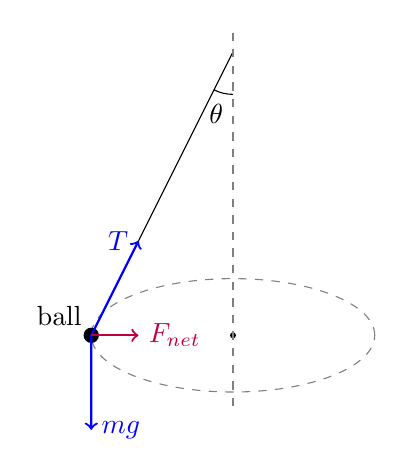
\begin{tikzpicture}[scale=0.6]
\draw [gray, dashed](0,0) ellipse (3 and 1.2);
\draw [fill] (0:-3) node[above left]{ball} circle [radius=0.15];
\draw [fill] (0:0) circle [radius=0.05];
\draw [blue,thick, <->] (-3,-2) node[right]{$mg$} -- (-3,0) --++ (1, 2) node[left]{$T$};
\draw [thick, ->, purple] (-3,0) -- (-2,0) node[right]{$F_\text{net}$};
\draw (-2, 2) -- (0,6) (0,5.1) node[below left]{$\theta$} arc(-90:-116.57:0.9);
\draw [gray, dashed] (0,-1.5) -- (0,6.5);
\end{tikzpicture}
\vspace*{5pt}
\end{marginfigure}

\begin{soln} vertical component of tension $T_y$ equals weight

{
	
	\centering

$T_y = mg \RA T\cos\theta = mg$

$T = \frac{mg}{\cos\theta} = \frac{0.12\times9.81}{\cos25^\circ} \approx 1.3 \text{ N}$

}

net force equals horizontal component of tension $T_x$

so component $T_x$ provides centripetal force

{
	
	\centering
	
	$F_c = T_x \RA T\sin\theta = \frac{mv^2}{r}$
	
}

by eliminating $T$ and $m$, one can find
\begin{equation*}
	v^2 = \frac{r\tan\theta}{g} = \frac{0.10\times\tan25^\circ}{9.81} \RA v \approx 0.069 \mps 
\end{equation*}
\end{soln}

\example{A small ball of mass $m$ is attached to an inextensible string of length $l$.  The ball is held with the string taut and horizontal and is then released from rest.}

\begin{marginfigure}
	\centering
	\vspace*{-8pt}
	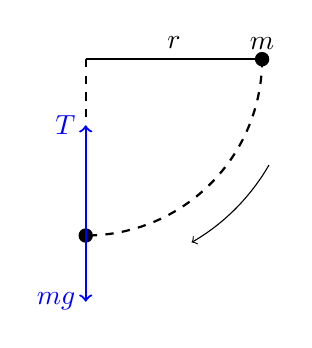
\begin{tikzpicture}[scale=0.56]
	\draw [thick, dashed] (0:4) arc [radius=4, start angle=0, end angle=-90];
	\draw [fill] (0:4) node[above]{$m$} circle [radius=0.15];
	\draw [fill] (-90:4) circle [radius=0.15];
	\draw [thick] (0,0) -- (2,0) node[above]{$r$} --(4,0);
	\draw [thick, dashed] (0,0) -- (0,-4);
	\draw [blue,thick,<->] (0,-1.5) node[left]{$T$} -- (0,-5.5) node[left]{$mg$};
	\draw [->] (-30:4.8) arc(-30:-60:4.8);
	\end{tikzpicture}
	\vspace*{45pt}
\end{marginfigure}

When the ball reaches lowest point, find its speed and the tension in the string in terms of $m$ and $l$.

\begin{soln} energy conservation: G.P.E. loss = K.E. gain
\begin{equation*}
	mgr = \frac{1}{2}mv^2 \quad \Rightarrow \quad v=\sqrt{2gr}
\end{equation*}

at lowest point: $\, F_c = T- mg = m \frac{v^2}{r}$
\begin{equation*}
	T = mg + m\frac{v^2}{r} = mg + m\frac{2gr}{r} = 3mg 
\end{equation*}
\end{soln}
\question{Suggest what provides centripetal force in the following cases. (a) An athlete running on a curved track. (b) An aeroplane banking at a constant altitude. (c) A satellite moving around the earth.}

\question{A turntable that can rotate freely in a horizontal plane is covered by dry mud. When the angular speed of rotation is gradually increased, state and explain whether the mud near edge of the plate or near the mud will first leave the plate?}

\question{A bucket of water is swung at a constant speed and the motion describes a circle of radius $r=1.0 $m in the vertical plane. If the water does not pour down from the bucket even when it is at the highest position, how fast do you need to swing the bucket?}
\begin{figure}
\begin{flushright}

	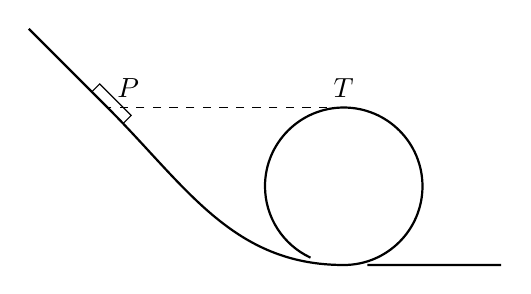
\begin{tikzpicture}
	\draw[thick] (-4,2) -- (-3,1) to [out=-45, in=180] (0,-1) arc[radius=1,start angle = -90, end angle = 245] (.3,-1) -- (2,-1);
	\draw[dashed] (0,1) node[above]{$T$} -- (-3,1) node[above right]{$P$};
	\draw (-3.2,1.2) -- ++(0.1,0.1) -- ++(0.4,-0.4) -- ++(-0.1,-0.1);
	\end{tikzpicture}
 \end{flushright}
\end{figure}

\question{This question is about the design of a roller-coaster. We consider a slider that starts from rest from a point $P$ and slides along a frictionless circular track as sketched below. $P$ is at the same height as the top of the track $T$. (a) Show that the slider cannot get to $T$. (b) As a designer for a roller-coaster, you have to make sure the slider can reach point $T$ and continue to slide along the track, what is the minimum height for the point of release?}
